%\setchapterimage{fig_00.jpg}
\chapter*{Application \arabic{cptApplication} \\ 
Machines Synchrones -- Alternateur
-- \ifprof Corrigé \else Sujet \fi}
\addcontentsline{toc}{section}{Application \arabic{cptApplication} : 
Machines Synchrones -- Alternateur
-- \ifprof Corrigé \else Sujet \fi}

\iflivret \stepcounter{cptApplication} \else
\ifprof  \stepcounter{cptApplication} \else \fi
\fi

\setcounter{question}{0}
\marginnote{Ressources de Philippe Dubois.}


Un alternateur triphasé dont les enroulements de stator sont couplés en étoile, fournit en charge nominale, un courant (efficace) $I = \SI{200}{A}$ sous une tension simple (efficace) $V = \SI{2,88}{kV}$ lorsque la charge est inductive et de facteur de puissance est égal à 0,87. 
La résistance d’un enroulement statorique vaut $R = \SI{0,20}{\Omega}$. 
La vitesse de rotation de la roue polaire est $N_S = \SI{750}{tr.min^{-1}}$.
Les tensions produites ont pour fréquence $f = \SI{50}{Hz}$. 
L’ensemble des pertes constantes et par effet Joule dans le rotor atteint \SI{55}{kW}. 
Un essai à vide, à la fréquence de rotation nominale, a donné les résultats suivants pour lesquels $I_e$ est l’intensité du courant d’excitation et $E_0$ la valeur efficace de la tension entre une phase et le neutre.


\begin{center}
\begin{tabular}{*{12}{c}}
\hline
$I_e$ (\si{A}) 	& 0	&10	& 20	& 30	& 40	& 50	& 60	& 70	& 80	& 90	& 100	\\
\hline
$E_0$ (\si{V})	& 0	& 606	& 1212	& 1819	& 2425	& 3002	& 3435	& 3782	& 4041	& 4215	& 4330	\\
\hline
\end{tabular}
\end{center}

Un essai en court-circuit a donné, pour un courant d´excitation d’intensité $I_e=\SI{40}{A}$, un courant dans les enroulements du stator $\indice{I}{cc}=\SI{2,5}{kA}$.

\question{Quel est le nombre de paires de pôles du rotor ?}
\ifprof
\begin{corrige}
On a $N_s = \dfrac{60f}{p}$ $\Rightarrow p = \dfrac{60f}{N_s}$ $=\dfrac{60\times 50}{750}=4$ paires de pôles.

\end{corrige}
\else
\fi

\question{Calculer la réactance synchrone $X_s$ de l’alternateur lorsqu’il n’est pas saturé.}
\ifprof
\begin{marginfigure}
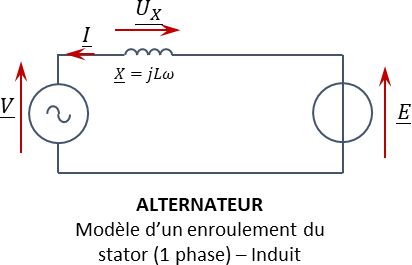
\includegraphics[width=\linewidth]{cor_02}

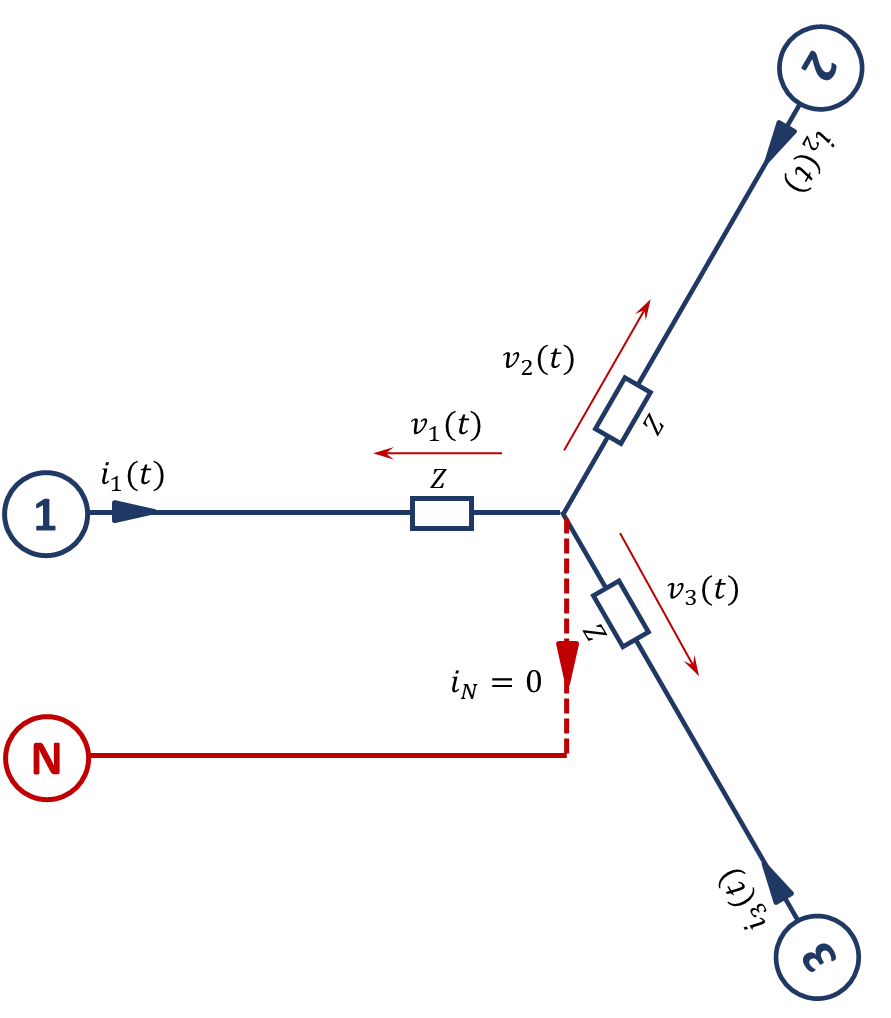
\includegraphics[width=\linewidth]{cor_03}
\end{marginfigure}
\begin{corrige}
Il s'agit d'un essai en court-circuit. 
On a $\underline{I}=\indice{I}{cc}\sqrt{2}e^{j\left(\omega t\right)}$.

Si le courant d'excitation du rotor est de $\SI{40}{A}$, alors $\underline{E}=E_0\sqrt{2}e^{j\left(\omega t + \varphi\right)}$ avec $E_0 = \SI{2425}{V}$.

Enfin, $\overline{U_X}=\indice{I}{cc}jL\omega\sqrt{2}e^{j\left(\omega t\right)}$


On a donc $E_0^2\sqrt{2}^2 = \left(\indice{I}{cc}L\omega\sqrt{2}\right)^2 + \left(R\indice{I}{cc}\sqrt{2}\right)^2$
$ \Rightarrow  E_0^2 = \indice{I}{cc}^2L^2\omega^2 + R^2\indice{I}{cc}^2$.

Ainsi, $L\omega = \sqrt{\dfrac{E_0^2-R^2\indice{I}{cc}^2}{\indice{I}{cc}^2}}$. \textit{AN :} $L\omega = \dfrac{\sqrt{2425^2-0,2^2\times 2500^2}}{2500} = \SI{0,95}{\Omega}$
\end{corrige}
\else
\fi

On supposera $X_s$ constante pour la suite.

\question{En déduire la f.e.m. synchrone $E$ au point de fonctionnement nominal et en déduire le courant d’excitation.}
\ifprof
\begin{marginfigure}
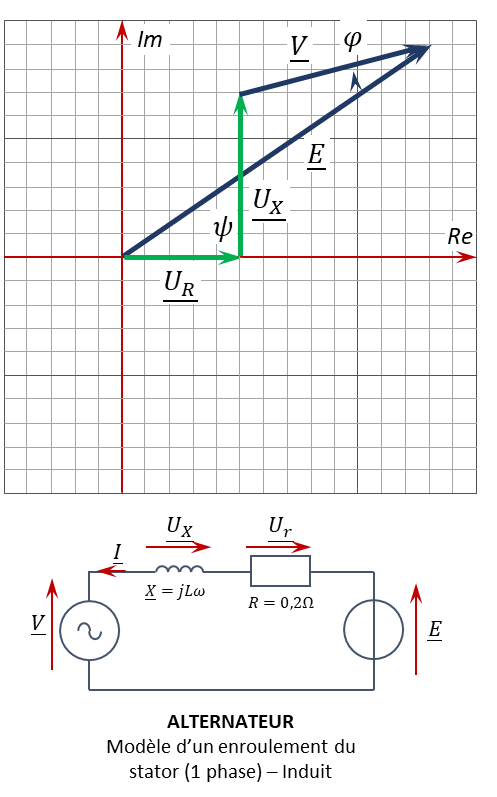
\includegraphics[width=\linewidth]{cor_04}
\end{marginfigure}
\begin{corrige}
On a maintenant $\underline{V}=V\sqrt{2}e^{j\left(\omega t + \varphi\right)}$ et 
$\underline{E}=E\sqrt{2}e^{j\left(\omega t + \psi\right)}$. (On cherche $E$, et $V = \SI{2,88}{kV}$.)

On a donc 
$\left\{
\begin{array}{l}
R\indice{I}{cc}\sqrt{2} + V\sqrt{2}\cos \varphi = E\sqrt{2} \cos \psi\\
\indice{I}{cc}\sqrt{2}L\omega + V\sqrt{2}\sin \varphi = E\sqrt{2} \sin\psi \\
\end{array}
\right.$

$\Rightarrow
E^2 = R^2\indice{I}{cc}^2 + V^2\cos^2 \varphi + 2R\indice{I}{cc}V\cos \varphi
+\indice{I}{cc}^2L^2\omega^2 + V^2\sin^2 \varphi
+2\indice{I}{cc}L\omega  V\sin \varphi
$

$\Rightarrow
E^2 = R^2\indice{I}{}^2 + V^2 
+\indice{I}{}^2L^2\omega^2 +2\indice{I}{}V\left(L\omega  \sin \varphi+ R\cos \varphi\right)
$



On a donc $E = \SI{3012}{V}$ et $I_e \simeq \SI{50}{A}$.
\end{corrige}
\else
\fi

\question{Calculer la puissance nominale fournie par l’alternateur et le rendement au point de fonctionnement nominal.}
\ifprof
\begin{corrige}

\end{corrige}
\else
\fi



\ifprof
\else
\begin{marginfigure}[-3cm]
\centering
%\includegraphics[width=3cm]{Cy_02_Ch_01_Activation_01_qr}
\end{marginfigure}
\fi




